% Copyright 2019 Clara Eleonore Pavillet

% Author: Clara Eleonore Pavillet (original author), Leonard Quentin Marcq (modified for Tsinghua), 赵宗义 (参与了修改)
% Description: This is an unofficial Tsinghua University Beamer Template I made from scratch. Feel free to use it, modify it, share it.
% Version: 1.1


\documentclass{beamer}
\usepackage{ctex}
\usepackage{fontspec}
% Load Packages
\usepackage[utf8]{inputenc}
\usepackage{xcolor}
\usepackage{tikz}
\usetikzlibrary{positioning,calc}
\usepackage{graphicx}
\usepackage{hyperref}
\usepackage{amsmath}
\usepackage{listings}
%\usepackage{fontawesome}

% Define Commands
\newcommand*{\ClipSep}{0.06cm} %To adjust footer logo
\newcommand{\E}{\mathrm{e}\,} %\def\I{e} % used to defined e for exp(x), see later what it should be
\newcommand{\ud}{\mathrm{d}}
\lstset{numbers=left, numberstyle=\tiny, stepnumber=1,firstnumber=1,breaklines=true,
    numbersep=5pt,language=Python,
    stringstyle=\ttfamily,
    basicstyle=\footnotesize, 
    showstringspaces=false
}

\usetheme{workhw}

%%%<<<---
\newcommand{\variable}{\mathrm}
\newcommand{\field}{\mathsf}
%%%--->>>

\title{容器集群降本增效}
%\titlegraphic{
\includegraphics[width=2cm]{Theme/Logos/tsinghua_emblem_dark.png}}
\author{刘欣}
%\institute{清华大学计算机科学与技术系}
\date{\today}

\begin{document}

{\setbeamertemplate{footline}{} 
\frame{\titlepage}}



\begin{frame}{主要内容}
\begin{itemize}
  \item \textbf{集群调度的核心挑战}
  \newline
%\begin{enumerate}
%\item 流记录项的分类和聚合
%\item 流记录项的存储和分析
%\end{enumerate}
  \item \textbf{集群调度技术演进}
  \newline
   \item \textbf{动态负载均衡服务落地实践}
  \newline
  \item \textbf{集群调度未来潜在演进方向}
  \newline
\end{itemize}
\end{frame}

\begin{frame}{集群调度的核心挑战}
\textbf{目标}
\begin{enumerate}
\item 整合离散和异构的服务器到弹性资源池,提高数据中心资源利用率,并提供自动化的运维能力。
\item 通过网络和存储系统,可以根据业务需求动态地分配计算实例,从而降低整体计算成本。
\end{enumerate}

\textbf{例如:} 
\newline
\setlength\parindent{24pt} \indent 按需为业务分配计算实例,并通过集群的规模效应降低计算成本

\end{frame}

\begin{frame}{集群调度技术演进}
\begin{enumerate}
\item 数据平面包含了两个哈希表, 分别是主表 (Main Table) 和辅表 (Ancillary Table).
\item 主表中每个哈希桶包含两个域: $\field{fieldID}$和$\field{count}$
\item 辅表中每个哈希桶也包含两个域: $\field{digest}$和$\field{count}$
\end{enumerate}
\begin{figure}
	\centering
	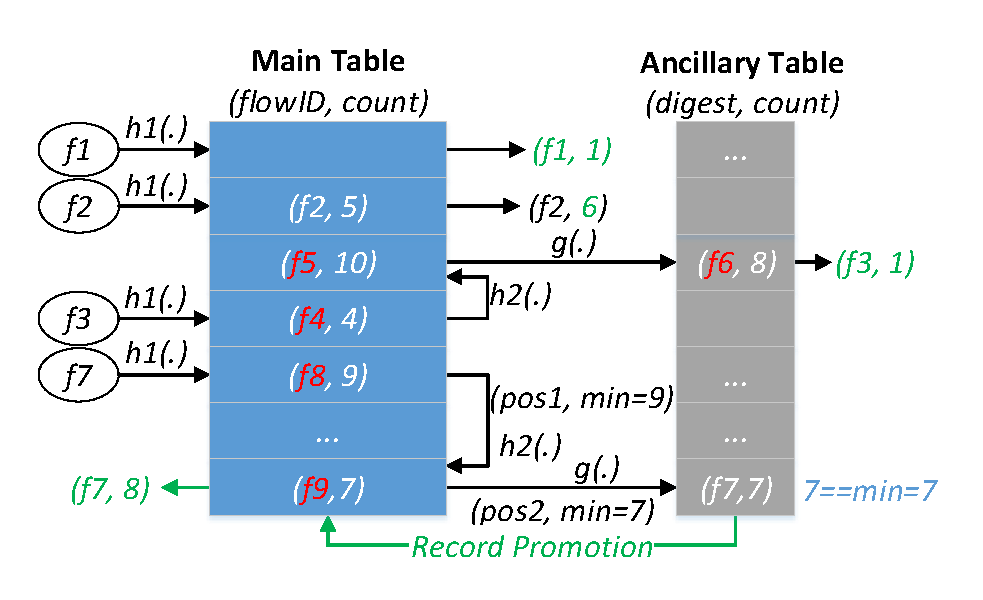
\includegraphics[width=0.6\linewidth]{figures/representation/datastructure}
\end{figure}

\end{frame}

\begin{frame}{动态负载均衡服务落地实践}
\begin{enumerate}
\item 数据平面包含了两个哈希表, 分别是主表 (Main Table) 和辅表 (Ancillary Table).
\item 主表中每个哈希桶包含两个域: $\field{fieldID}$和$\field{count}$
\item 辅表中每个哈希桶也包含两个域: $\field{digest}$和$\field{count}$
\end{enumerate}
\begin{figure}
	\centering
	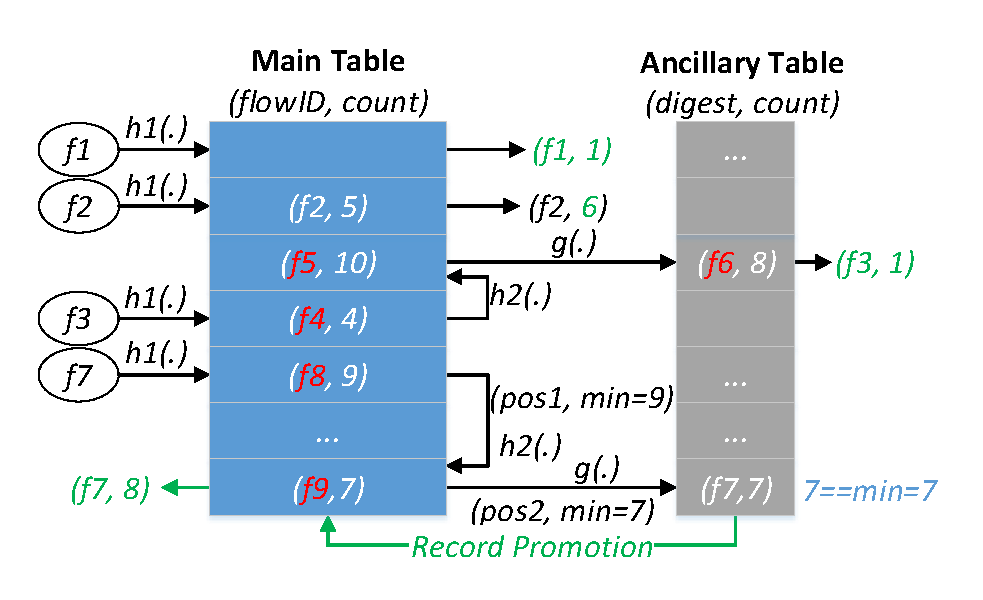
\includegraphics[width=0.6\linewidth]{figures/representation/datastructure}
\end{figure}

\end{frame}

\begin{frame}{集群调度未来潜在演进方向}
\begin{enumerate}
\item 数据平面包含了两个哈希表, 分别是主表 (Main Table) 和辅表 (Ancillary Table).
\item 主表中每个哈希桶包含两个域: $\field{fieldID}$和$\field{count}$
\item 辅表中每个哈希桶也包含两个域: $\field{digest}$和$\field{count}$
\end{enumerate}
\begin{figure}
	\centering
	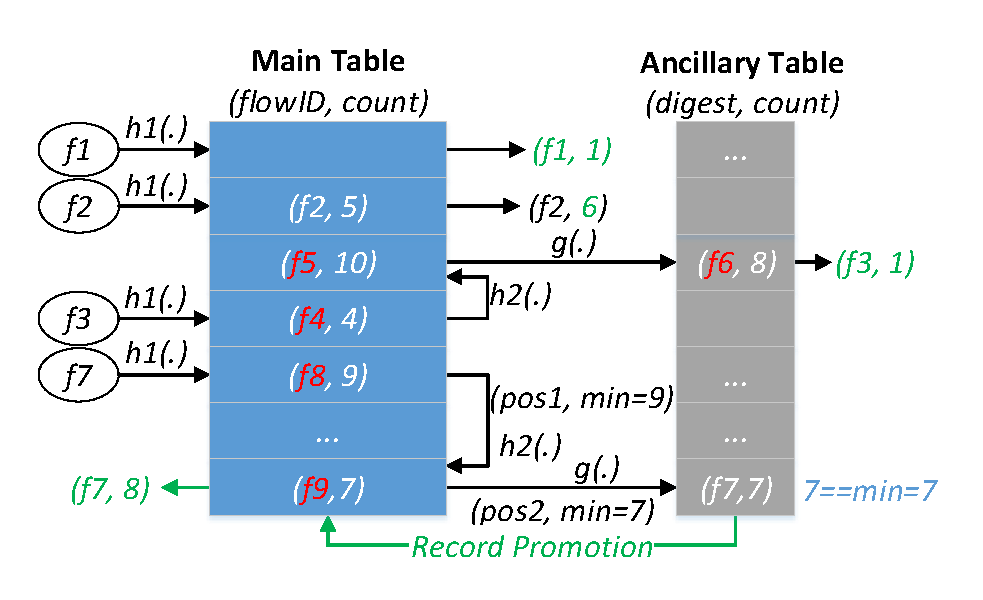
\includegraphics[width=0.6\linewidth]{figures/representation/datastructure}
\end{figure}

\end{frame}

  
\begin{frame}{}
\begin{center}
    \textbf{谢谢!}
\end{center}
\end{frame}


\end{document}

